\documentclass[12pt,a4paper,fleqn]{report}
\usepackage[utf8]{inputenc}
\usepackage[brazil]{babel}
\usepackage{graphicx}
\usepackage{hyperref}
\usepackage{abnt-alf}
\usepackage[top=3cm,bottom=2cm,left=3cm,right=2cm]{geometry}
\usepackage{color,colortbl,multirow}
\usepackage{indentfirst}
\usepackage{mathtools}
\usepackage{dsfont}
\usepackage{amssymb}
\usepackage{amsfonts}
\usepackage{amsthm}
\usepackage{amsmath}
\usepackage{longtable}
\usepackage{float}
\usepackage{epigraph}
\usepackage{url}
\usepackage{pdfpages}
\usepackage[portuguese]{nomencl}
\makenomenclature
\author{Brian Lee Mayer, Luiz Henrique Alves Monteiro}
%\numberwithin{equation}{subsection}

\begin{document}

% CAPA
\pagestyle{empty}
\begin{center}
\large  \textbf{UNIVERSIDADE PRESBITERIANA MACKENZIE}
\large  \textbf{PROGRAMA DE PÓS-GRADUAÇÃO EM}\\
\large  \textbf{ENGENHARIA ELÉTRICA E COMPUTAÇÃO}\\
\vskip 2.0cm
\textbf{\large Brian Lee Mayer}\\
\vskip 3.5cm
\setlength{\baselineskip}{1.5 \baselineskip}
\textbf{\large INVESTIGANDO NÚMEROS PRIMOS \break COM ALGORITMOS DE VISIBILIDADE}\\
\vskip 3.5cm
\end{center}
\hfill{\vbox{\hsize=10cm\noindent\strut
Projeto de qualificação de doutorado 
apresentado ao Programa de 
Pós-Graduação em Engenharia Elétrica e
Computação da Universidade
Presbiteriana \mbox{Mackenzie} como requisito
para a obtenção do grau de Doutor
em Engenharia Elétrica e Computação}
\strut}
\vskip 2.0cm
\textbf{\normalsize \raggedright Orientador: 
Dr. Luiz Henrique Alves Monteiro}
\vskip 2.0cm
\begin{center}
São Paulo\\
2022\\
\end{center}
% \includepdf{Ficha/ficha_Gina Szajnbok Harari_V18.pdf} % inclui a Ficha Catalográfica
\newpage
% \includepdf{Aprovacao/aprovacao_Gina Szajnbok Harari_V18.pdf} % inclui a Ficha Catalográfica
\newpage
% \includepdf{Fomento/fomento_Gina Szajnbok Harari_V18.pdf} % inclui a Ficha Agencia Fomento (Bolsa)

\newpage
% RESUMO
\thispagestyle{plain}
\pagenumbering{roman}
\begin{center}
\large
\textbf{RESUMO}
\end{center}
\renewcommand{\baselinestretch}{0.6666666}

Seja $d$-primo um número natural com exatamente $d$ divisores. De acordo com essa definição, os números primos usuais
correspondem ao caso particular $d=2$. Parte deste trabalho consiste em investigar numericamente as  
sequências numéricas que correspondem às lacunas entre  $d$-primos consecutivos, com $d \in \{2,3,,...,11\}$. A partir dessas sequências, grafos são construídos usando algoritmos de visibilidade natural e de visibilidade horizontal e, então, as topologias desses grafos são analisadas. Nessas análises, calcula-se também a entropia informacional das sequências de lacunas e a densidade dos $d$-primos. As simulações computacionais
mostraram que os grafos gerados a partir das lacunas entre $d$-primos consecutivos têm, em geral, uma distribuição de graus que é livre de escala. Essas simulações também mostraram que a densidade de $d$-primos para $d$ par é muito maior do que para $d$ ímpar e que a entropia informacional é maior para $d$ ímpar do que para $d$ par, para 
$d \in \{2,3,,...,11\}$. Neste trabalho, analisam-se ainda os grafos de visibilidade natural e de visibilidade horizontal gerados por sequências 
formadas a partir da quantidade de divisores dos números naturais e por sequências
obtidas a partir das casas decimais de números irracionais.


\noindent
{\bf Palavras-chave:} {\it algoritmo de visibilidade, $d$-primo, entropia informacional, rede complexa, sequência numérica.}


\newpage

% SUMÁRIO
\newpage
\thispagestyle{empty}
\tableofcontents
\listoffigures
\listoftables

% INTRODUÇÃO
\newpage
\pagestyle{plain}
\pagenumbering{arabic}
\renewcommand{\baselinestretch}{1.5}
\normalsize


\chapter{INTRODUÇÃO}

Um número primo é um número natural maior do que 1 que possui apenas dois divisores: o número 1 e ele próprio. 
Desde a Antiguidade, os números primos têm fascinado os matemáticos e entusiastas
da Matemática \cite{a66,a44} e atraído a atenção de
grandes mentes, como  Eratóstenes, Erd\"os, Euclides, 
Euler, Fermat,  Gauss e Riemann \cite{a66,a44}. A primeira
referência a um algoritmo para descobrir os números primos dentro de uma sequência numérica foi o crivo de Eratóstenes \cite{nicomachus300}, proposto por volta de 250 aC. Esse crivo funciona da
seguinte maneira. Suponha que se deseja encontrar todos os primos menores
ou iguais a $n$. Para isso:

\begin{enumerate}
    \item crie uma lista de inteiros consecutivos de 2 até $n$;
    \item inicialmente, tome $p = 2$, o primeiro número primo;
    \item elimine todos os  múltiplos de $p$ até o fim da lista;
    \item considere o próximo número que não foi eliminado (no caso, $p=3$) e repita o passo anterior;
    \item repita o passo 3, considerando o próximo número da lista (no caso, $p=5$);
    \item repita o passo 3 até que não haja
    número eliminado. Quando isso ocorrer, pare. Ao final da execução desse algoritmo, os números que não foram eliminados são primos.
\end{enumerate}
    


Os números primos são conhecidos por serem fundamentais em estudos
em muitas áreas, como a Teoria dos Números \cite{a66,a44}.
Na Matemática Aplicada, os números primos são usados em criptografia
\cite{a65}. Um exemplo clássico  é o sistema de criptografia
conhecido como RSA (em homenagem a Rivest, Shamir e Adleman), que se baseia na dificuldade prática de se fatorar
números com muitos dígitos (da ordem de centenas ou milhares de bits). Na Biologia, algumas espécies de cigarras possuem ciclo de vida
cuja duração é um número primo de anos, como 13 ou 17 anos, provavelmente como estratégia de sobrevivência \cite{a48}. Na Física, os primos caracterizam o espectro de energia de sistemas 
quânticos caóticos \cite{a59}. 

Se um número natural não é primo, então ele é composto.
O Teorema Fundamental da Aritmética, que remete aos trabalhos de Euclides, feitos por volta de 300 aC, estabelece que qualquer número natural possui uma única decomposição em fatores primos. Por exemplo, $4044=2^2 \times 3^1 \times 337^1$. Talvez os números primos tenham ganhado esse nome porque são números primários, ou seja, os números a partir dos quais se escrevem os demais. Acredita-se que o conceito de número primo se deve a Euclides, por volta de 300 aC \cite{garbi09}. Em meados do século XIX, Kulik determinou, a mão, os primos até 100.000.000 \cite{kulik83}. As tabelas anteriores listavam os primos até 100.000.

%As sequências de primos, por sua irregularidade, são um campo de estudos
%por si só e têm sido investigadas por muitos séculos \cite{a44,g01,t16}.
%Um estudo proeminente é usar grafos para estudar as relações entre os
%números, por exemplo, se os números primos são representados como nós de
%um grafo, então se dois primos tem como soma um número par, eles estariam
%ligados, como na conjectura de Goldbach \cite{a04}.


Gauss, um dos maiores matemáticos de todos os tempos, paralelamente a Legendre,
por volta de 1800 \cite{d05}, conjecturou a respeito da função  contagem de números
primos, denotada por $\Pi(n)$, que expressa a quantidade de primos menores ou iguais a $n$. Para Gauss, $\Pi(n)$
se aproxima de:
$$\frac{n}{\ln(n)}$$
para $n \to \infty$. Ou seja:
$$\lim_{n\to \infty}\frac{\Pi(n)}{n/\ln(n)} = 1$$

\noindent
Por exemplo, para $n=10$, $\Pi(10)=4$ (pois há quatro primos menores do que 10) e 
$10/\ln(10) \simeq 4,34$; logo,
$\Pi(10)/[10/\ln(10)] \simeq 0,92$; para $n=10^{10}$, $\Pi(10^{10})=455052511$ e $10^{10}/\ln(10^{10}) \simeq 4,34 \times 10^8$; logo $\Pi(10^{10})/[10^{10}/\ln(10^{10})] \simeq 1,05$. Para Legendre,
no lugar de $\ln(n)$, escreve-se $\ln(n)-1,08$.
Desde esses trabalhos de Gauss e Legendre, a fórmula para $\Pi(n)$ continuou sendo investigada, por exemplo, por Chebyshev \cite{t16}. Hadamard provou, por volta de 1900, que a fórmula proposta por Gauss é a correta \cite{ken98}. Erd\"os, nos anos 50 do século passado, apresentou uma prova mais simples desse resultado \cite{ten}.

Em 1737, Euler encontrou uma identidade que relaciona os números primos com a função $\zeta(s)$,
hoje conhecida como função zeta de Euler-Riemman, dada por:
$$
\zeta(s) = \frac{1}{1^s} + \frac{1}{2^s} + \frac{1}{3^s} +
\frac{1}{4^s} + ...
$$
\noindent em que $s$ \'e um número real. Euler mostrou que $\zeta(s)$ também se escreve como:
$$
\zeta(s) = \frac{1}{(1-(1/2^s))} \frac{1}{(1-(1/3^s))}  \frac{1}{(1-(1/5^s))} 
\frac{1}{(1-(1/7^s))}  ...
$$

\noindent Essa identidade é chamada de
formula do produto para a função zeta. Tomando $s=1$,
Euler provou que há infinitos números primos \cite{ten}.

Em 1859, Riemman
publicou um artigo 
%cuja primeira página é mostrada na Figura 1.1, 
que considera $s$ em $\zeta(s)$ como sendo um número complexo \cite{ten}. Esse artigo também contém a famosa Hipótese de Riemann, um dos problemas abertos da Matemática
Pura mais importantes de todos os tempos. Essa hipótese relaciona as raízes complexas da função $\zeta(s)$ com a possibilidade de se calcular $\Pi(n)$ a partir de $\zeta(s)$.
 
%\begin{figure}[h!]
 %   \centering
  %  \includegraphics[width=0.5\t%extwidth]{Images/riemman.png}
   % \caption{ Recorte da %primeira página do ``Ueber %die Anzahl der Primzahlen %unter einer
%gegebenen Grösse''. Fonte: %Wikipedia}
 %   \label{riemman}
%\end{figure}

%Um trabalho moderno na mesma área é de \cite{hutama17}, que implementa
%em \emph{software} as fórmulas explicitas de Riemman para primos racionais e gaussianos.

Um dos sonhos dos matemáticos é encontrar uma fórmula que preveja corretamente a sequência de todos os números primos. Inspirado por esse objetivo, 
Euler propôs uma função polinomial $P(n)$ capaz de gerar muitos números primos. Essa função é dada por:
$$P(n) = n^2 - n + 41$$
\noindent Essa fórmula gera primos para $n=1,\ldots,40$, falha para $n=41$ e $42$, mas continua gerando alguns
primos para $n>42$.

Existem muitos outros polinômios geradores de primos; no entanto, nenhum deles gera apenas
números primos. Há, por exemplo, os primos de Mersenne que são obtidos de \cite{ten}:
$$M(n)=2^n-1$$
\noindent Por exemplo, $M(2)=3$, $M(3)=7$ e $M(5)=31$ são primos, mas $M(4)=15$ não é. Os maiores números primos conhecidos são primos de Mersenne. Até o momento, o maior primo foi encontrado em 2018 e é dado por $M(82589933)$ \cite{primes}.

Por volta de 1650, Fermat conjecturou, numa carta para Mersenne, que $2^{2^n}+1$
daria sempre números primos, mas essa fórmula falha para $n=5$, como mostrado por Euler \cite{ten}.

%Existe uma conexão entre esses polinômios geradores de primos e um recente
%resultado de \cite{greentao}.

A lacuna entre números primos, ou seja, o intervalo entre primos consecutivos, é outro assunto que tem
recebido atenção ao longo dos anos \cite{e35,g01},
Nesses estudos, busca-se caracterizar as propriedades estatísticas da distribuição das lacunas
entre primos sucessivos, da distribuição das lacunas entre as lacunas, ou seja, das lacunas de segunda ordem, e das lacunas de ordens superiores \cite{a05,a02}. Num outro estudo  \cite{t16}, deduziu-se uma fórmula para a lacuna máxima
entre dois primos.

As distribuições dos números primos também têm sido estudadas usando grafos. Por exemplo, considere que
os nós de um grafo são números primos. De acordo com 
a conjectura de Goldbach,
qualquer número par pode ser
escrito como a soma de dois primos. Assuma que dois nós (dois primos) estão
ligados se a soma deles representa um número par \cite{a04}. Nesse trabalho, analisou-se o grafo assim gerado, considerando que  diversos números pares podem ser representados pela soma de diferentes primos (por exemplo 22=3+19=5+17). Em outro estudo com grafos, os números naturais são os nós
e uma ligação é adicionada entre dois nós se eles possuem um divisor comum que é
primo \cite{a16}. 

Nesta tese, analisam-se sequências de $d$-primos por meio de grafos. Aqui, define-se um $d$-primo como um número natural que tem exatamente $d$-divisores.
Usando essa definição, é evidente que os números primos são o caso particular 
$d=2$. 
A intenção deste estudo baseado em $d$-primos é explorar como
as sequências de lacunas
variam com $d$, com $d \in \{2,3,\ldots,11\}$. Para isso, convertem-se essas sequências em grafos por meio de algoritmos de visibilidade \cite{a14,a13}.
Para os grafos assim gerados, determinam-se a distribuição de grau e o grau médio. Ainda, a variabilidade dessas sequências é avaliada calculando a entropia informacional \cite{a301}. A densidade de $d$-primos, dada por $\Pi_d(n)/n$, também é computada. Outros experimentos numéricos envolvendo números irracionais e os divisores dos números naturais são também realizados. 

Este texto está assim organizado. No capítulo 2, apresentam-se definições básicas e os algoritmos utilizados nesta tese. No capítulo 3, descrevem-se os estudos numéricos realizados. No capítulo 4, mostram-se os resultados  obtidos nesses estudos. No capítulo 5, listam-se as conclusões preliminares e os próximos passos para finalizar esta tese. 



\chapter{DEFINIÇÕES E MÉTODOS}

Neste capítulo, são apresentados os conceitos, as fórmulas e os algoritmos necessários
para os estudos numéricos realizados neste trabalho. Alguns desses conceitos já foram mencionados no capítulo anterior.

\section{Definições}

\subsection{Sequência}

Ao longo deste trabalho, o termo sequência aparece diversas vezes, sendo
uma definição necessária para um melhor entendimento desse conceito.

\paragraph*{Definição:}

Uma sequência de números reais é uma função $x(n):\mathbb{N}\to\mathbb{R}$.
\cite{lima76}, que atribui um número real $x$ a cada posição de uma lista, sendo essa posição identificada por um número natural $n$. Assim, $x(n)$ corresponde ao  $n$-ésimo valor de $x$ 
da sequência $\{x(1),x(2),x(3),\ldots\}$. Note que esse conjunto  possui ordem
definida.

%$(x)_{n\in\mathbb{N}}$, ou $(x_n)$ para indicarmos
%a sequencia $(x_1,x_2,x_3,\ldots, x_n,\ldots)$, note a diferença para o
%conjunto $\{x_1,x_2,x_3,\ldots, x_n,\ldots\}$, a sequencia possui ordem
%definida.

%\subsection{Operador diferença}

%Uma operação básica que é utilizada ao longo deste trabalho é a diferença. Aqui,
%usa-se a notação $\Delta$ por ser a mais usual.

%\paragraph{Definição:}

%Seja $f(x)$ uma função de $x$ e $h$ uma constante tal que $x+h$ pertence ao domínio
%de $f$. Admita que  $\Delta f(x)$ denote a primeira diferença de $f(x)$. Calcula-se $\Delta f(x)$ por meio da expressão
%$\Delta f(x) = f(x+h) - f(x)$ \cite{goldberg86}.

\subsection{Número primo}

A definição de número primo é apresentada em diversos  livros
de matemática básica.

\paragraph*{Definição:} Um número primo é um número natural maior do que 1 e que possui
nenhum outro divisor além de 1 e de si mesmo \cite{knuth}.


\subsection{Teorema Fundamental da Aritmética}

O Teorema Fundamental da Aritmética fornece o alicerce central para a construção dos números naturais e para a fatoração prima.

\paragraph*{Definição:} Todo natural $n > 1$ ou é primo ou é um produto
de números primos. Assim, $n$ possui uma representação única, desconsiderando a ordem
dos fatores, e pode ser escrito como $n = p_1 ^a\times p_2 ^b\times p_3^c,\ldots$ sendo 
$p_1, p_2, p_3,\ldots$ seus fatores primos e $a, b, c, \ldots$ as respectivas multiplicidades desses fatores \cite{ten}. 

A noção apresentada a seguir está intimamente relacionada com o teorema exposto acima. Apesar de simples e natural, a ideia de $d$-primo não foi encontrada na literatura.


\subsection{Número $d$-primo}

Assim como um número primo possui exatamente 2 divisores, pode-se estabelecer que um número chamado de
$3$-primo possui exatamente 3 divisores. Por exemplo, 4 é 3-primo, pois seus divisores
são 1, 2 e 4. Generalizando, um $d$-primo possui exatamente $d$ divisores.

\paragraph*{Definição:} Um $d$-primo é um número natural  que possui exatamente
$d$ divisores.

Note que, pela definição acima, os $2$-primos correspondem aos números primos usuais. A sequência de 2-primos começa com 2, 3, 5, 7, 11, 13, 17, 19,\ldots, pois esses números possuem apenas dois divisores.
Note também que não há controvérsia ao afirmar que 1 é 1-primo, segundo 
a definição de $d$-primo.
Portanto, nossa definição de $d$-primo nada mais é do que uma generalização baseada na quantidade de divisores de um número natural.

Aqui, usa-se a notação $p_d(n)$ para designar o $n$-ésimo $d$-primo, com $n \in \mathbb{N}^*$.
Dessa forma, $p_3(4)$ é o quarto 3-primo, que é o número 49. A Tabela 2.1 
apresenta os primeiros $d$-primos para $d=\{2, 3, \ldots, 11\}$. 


\begin{table}[ht]
\begin{center}
\caption{Sequências de $d$-primos, denotadas por $p_d(n)$.}

\vskip 1cm
\begin{tabular}{|c|l|} \hline
        $d$ & $p_d(n)$ \\
        \hline
        2 & $2, 3, 5, 7, 11, 13, 17, 19, 23, 29, 31, 37, 41, \ldots$ \\
        3 & $4, 9, 25, 49, 121, 169, 289, 361, 529, 841, \ldots$ \\
        4 & $6, 8, 10, 14, 15, 21, 22, 26, 27, 33, 34, 35, \ldots$ \\
        5 & $16, 81, 625, 2401, 14641, 28561, 83521, \ldots$ \\
        6 & $12, 18, 20, 28, 32, 44, 45, 50, 52, 63, 68, 75 \ldots$ \\
        7 & $64, 729, 15625, 117649, 1771561, 4826809, \ldots$ \\
        8 & $24, 30, 40, 42, 54, 56, 66, 70, 78, 88, 102, \ldots$ \\
        9 & $36, 100, 196, 225, 256, 441, 484, 676, 1089, \ldots$ \\
        10 & $48, 80, 112, 162, 176, 208, 272, 304, 368, \ldots$ \\
        11 & $ 1024, 59049, 9765625, 282475249, \ldots$ \\
        \hline
    \end{tabular}
    \label{tab:n-primes}
\end{center}
\end{table}

\subsection*{Contagem de $d$-primos}

Assim como o conceito de $d$-primo é uma extensão do conceito de primo, a função 
contagem de $d$-primos $\Pi_d(n)$ é uma extensão da  função contagem de primos $\Pi(n)$.

\paragraph*{Definição:} A função  contagem de $d$-primos, representada por
$\Pi_d(n)$, com $n\in \mathbb{N}$, é definida como o número de $d$-primos
menores ou iguais a $n$.

Portanto, $\Pi_2(n)$ equivale à usual função  contagem de primos. Por exemplo, $\Pi_2(10) = 4$, pois só há quatro 2-primos menores ou
iguais a 10 (os números 2, 3, 5 e 7). Já $\Pi_3(10) = 2$, pois apenas 4 e 9 são 3-primos menores ou iguais a 10.

\subsection{Função quantidade de divisores}

\paragraph*{Definição:} A função quantidade de divisores $D(n): 
\mathbb{N}\to\mathbb{N}$
é tal que $D(n)=d$, sendo $d$ o número de divisores do número natural $n$.

Por exemplo, $D(2)=2$ e $D(4)=3$.

\subsection{Entropia informacional}

A variabilidade de uma sequência $x(n)$ pode ser avaliada calculando a entropia  $H$ proposta por Shannon. Quanto maior a variabilidade dos valores de $x(n)$, maior $H$.


\paragraph*{Definição:} A entropia informacional $H$ é definida como 
$H=-\sum_{i=1}^q \rho_i \ln \rho_i$, sendo $\rho_i$ a frequência relativa com que aparece o $i$-ésimo 
valor de $x$ na sequência $x(n)$, sendo $q$ o número de valores de $x$ que são distintos. O máximo de $H$ vale $H_{max}=\ln q$, 
que é obtido no caso em que $p_i=1/q$ para
$i=1, \ldots, q$; ou seja, a entropia máxima corresponde ao caso em que todos os valores de $x$ aparecem nessa sequência com mesma frequência relativa \cite{a301}.

Essa entropia tem sido utilizada em diversos trabalhos envolvendo, por exemplo, a dinâmica de sistemas biológicos e sociais \cite{a305,a302}. Ela ainda pode empregada como uma medida de complexidade. 

\paragraph*{Definição:} A complexidade $C_{SDL}$ \cite{sdl} de uma sequência é calculada por $C_{SDL}=h(1-h)$, sendo $h=H/H_{max}$. 

Portanto, $C_{SDL}$ é máxima para $h=1/2$. Ou seja, a complexidade máxima ocorre entre a entropia mínima $H=0$ e a entropia máxima $H_{max}$.

\subsection{Lei de potência}

\paragraph*{Definição:} Uma lei de potência é uma função $f(x)$ que se relaciona com sua variável $x$ por meio da fórmula $f(x)=A x^{-\gamma}$, com $A$ e $\gamma$ constantes \cite{a83}.

Uma lei de potência é livre de escala, pois trocando $x$ por $Bx$, sendo $B$ uma constante, a relação entre $f(x)$ e $x$ não muda. De fato, $f(Bx)=A(Bx)^{-\gamma}=A^{'}x^{-\gamma}$, com $A^{'}=AB^{-\gamma}$. Portanto, a mudança de escala em $x$ altera apenas a constante multiplicativa (de $A$ para $A^{'}$), sem alterar a dependência com $x$ (que, no caso, é do tipo $x^{-\gamma}$).

Num gráfico log-log,
uma lei de potência corresponde a uma equação de reta, pois 
$\log f(x) = \log A - \gamma \log x$. Assim, $\log f(x)$ varia linearmente com $\log x$, de modo que o coeficiente angular dessa reta vale $-\gamma$

Nesta tese, usa-se uma lei de potência para ajustar a distribuição de graus dos grafos obtidos 
por meio dos algoritmos de visibilidade descritos a seguir. 


\section{Métodos}

Aqui são apresentados dois algoritmos que convertem
séries temporais em grafos não direcionados \cite{a14,a13}.
Esses algoritmos têm sido usados, por exemplo, em análises de ações de bolsa de valores 
\cite{a94} e de  eletroencefalogramas \cite{b01}. Eles são chamados de algoritmo de visibilidade natural e algoritmo de visibilidade horizontal.

\subsection{Visibilidade natural}

Seja a sequência (ou a série temporal) $\{x(1), x(2), x(3),...\}$. Assuma que $a < i < b$. No grafo de visibilidade natural (VN)
\cite{a14}, obtido a partir da sequência $x(n)$, com $n=1,2,3,...$,
os nós $x(a)$ e $x(b)$ estão conectados se todos os pontos intermediários $(i,x(i))$ estão abaixo da reta
que liga os pontos $(a,x(a))$ e $(b,x(b))$. 

\begin{figure}[h]
    \centering
    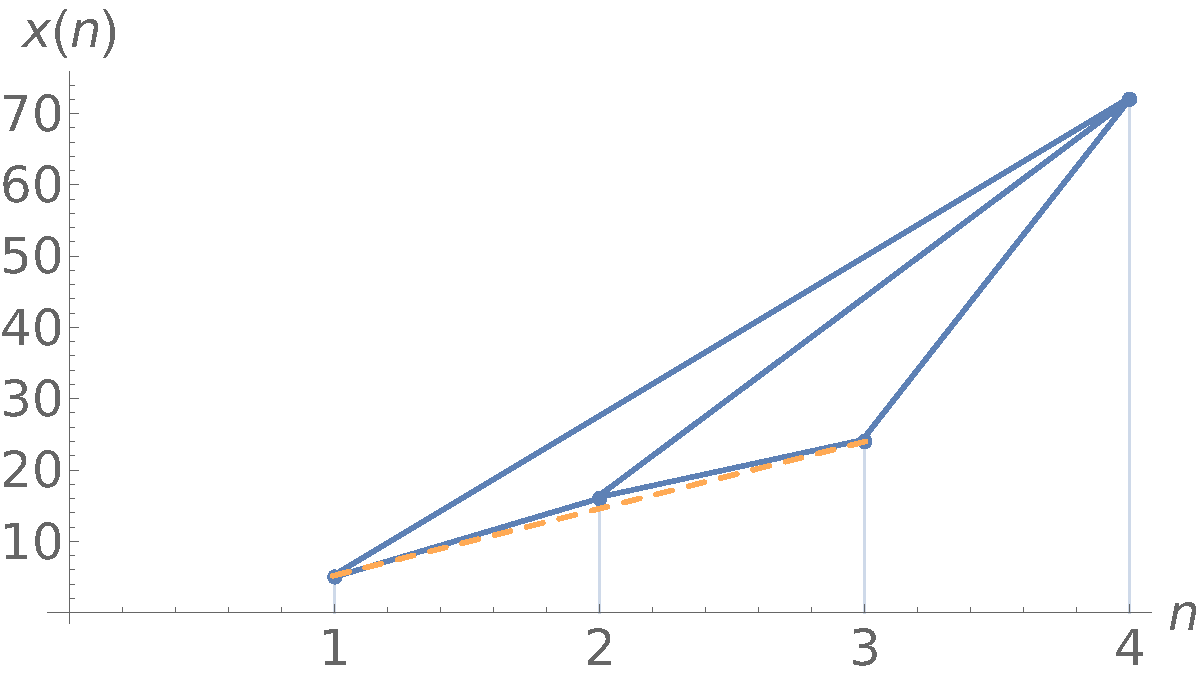
\includegraphics[width=270px]{Images/example-plot-natural.pdf}
    \caption{A sequência $x(n)$ em função de $n$, com $x(1)=5$, $x(2)=16$, $x(3)=24$ e
$x(4)=72$.}
\end{figure}

Por exemplo, suponha que os quatro primeiros
pontos de uma sequência $x(n)$ sejam $x(1)=5$, $x(2)=16$, $x(3)=24$ e
$x(4)=72$, como ilustra a 
Figura 2.1. No grafo de VN correspondente a essa sequência, existe uma conexão entre os nós 16 e 72, pois 
o único ponto intermediário $x(3)=24$ está abaixo da reta que liga 
$x(2)=16$ e
$x(4)=72$. Já os pontos $x(1)=5$ e $x(3)=24$ não estão conectados, pois  $x(2)=16$ está acima da reta que passa por esses dois pontos.


\begin{figure}[h]
    \centering
    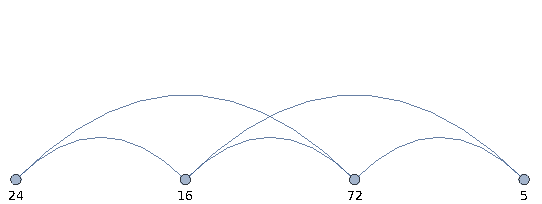
\includegraphics[width=320px]{Images/example-graph-natural.pdf}
    \caption{Grafo de VN gerado a partir da sequência mostrada na Figura 2.1.}
\end{figure}

\paragraph*{Método:} Sejam $a$, $b$ e $i$ indices de uma sequência
$x(n)$, com  $a < i < b$. No grafo de visibilidade
natural (VN), $x(a)$ e $x(b)$ estão conectados se todos os pontos
intermediários $(i, x(i))$  satisfazem a desigualdade \cite{a14}:
\begin{equation}
\label{nv}
x(i) < x(a) + \left( x(b)-x(a) \right) \left(
\frac{i - a}{b-a} \right)
\end{equation}

\noindent
Em outras palavras,  os nós $x(a)$ e $x(b)$ estão ligados se existe uma reta
passando por $(a,x_a)$ e $(b,x_b)$ no gráfico $x(n) \times n$, tal que nenhum ponto
intermediário está acima dessa reta ou coincide com ela.
No exemplo dado da Figura 2.1, como
$x(3)= 24 < x(2) + (x(4)-x(2)) (3-2)/(4-2)= 16 + (72-16)/2 = 44$, então os nós 16 e 72 estão conectados. Por outro lado, como
$x(2)=16 > x(1) +
(x(3)-x(1))(2-1)/(3-1) = 5 + (24-5)/2 = 14.5$, então os nós 5 e 24 não estão conectados. Nesse caso, o ponto $(2,16)$
é alto o suficiente para impedir que os pontos $(1,5)$ e $(3,24)$
se ``vejam".

A Figura 2.2 mostra o grafo gerado usando a Equação (2.1) para a sequência correspondente à Figura 2.1.


\subsection{Visibilidade horizontal}

No grafo de visibilidade horizontal (VH) \cite{a13}, os nós
$x(a)$ e $x(b)$ estão conectados se
todos os pontos intermediários $(i,x(i))$ no gráfico $x(n) \times
n$ estão abaixo da linha horizontal que une  $(a, x(a))$ e
$(b,x(b))$. 

\begin{figure}[h]
    \centering
    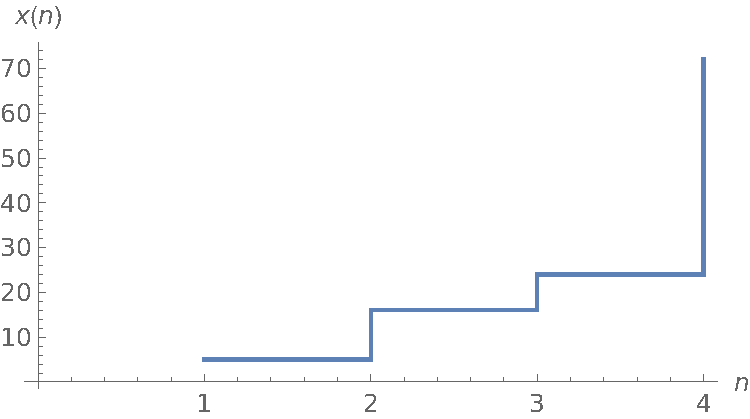
\includegraphics[width=270px]{Images/example-plot-horizontal.pdf}
    \caption{A sequência x(n) em função de n, com $x(1) = 5$, $x(2) = 16$, $x(3) = 24$ e
$x(4) = 72$.}
\end{figure}

Tomando a mesma sequência usada para exemplificar VH, os nós $x=16$ e $x=72$
não estão conectados, pois $x(2)=16<x(3)=24$; isto é, $(2,16)$
e $(4,72)$ não veem se olharem apenas na direção horizontal, pois o ponto intermediário $(3,24)$
é suficientemente alto para bloquear a visibilidade horizontal. Esse exemplo ilustra a
diferença entre as duas visibilidades, pois  pontos que  estão conectados
no grafo de VN podem não estar conectados no grafo de VH. Na verdade, o grafo de VH é um subgrafo do grafo de VN \cite{a13}.

\begin{figure}[h]
    \centering
    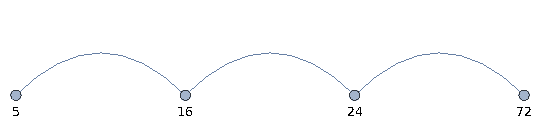
\includegraphics[width=320px]{Images/example-graph-horizontal.pdf}
    \caption{Grafo de VH gerado a partir da sequência mostrada na Figura 2.3.}
\end{figure}

\paragraph*{Método:} Sejam $a$, $b$ e $i$ indices de uma sequência
$x(n)$, com  $a < i < b$. No grafo de visibilidade horizontal (VH), obtido a partir da sequência $x(n)$, com $n=1,2,3,...$, os nós $x(a)$ e $x(b)$ estão conectados se todos os pontos intermediários $(i,x(i))$ satisfazem a desigualdade \cite{a13}:
\begin{equation}
\label{hv}
\left\{ x_a, x_b \right\} > x_i
\end{equation}

\noindent Assim,
dois nós estão conectados se nenhum ponto intermediário
está acima deles.

A Figura 2.4 mostra o grafo gerado usando a Equação (2.2) para a sequência correspondente à Figura 2.3.



\section{Relação entre $d$-primos e $d$ primo}

Como já mencionado, qualquer número natural pode ser fatorado como o produto de
 fatores primos. %colocar ref.
No caso particular de um número primo, seus fatores são 1 e o próprio número. Seja $p_2$ um primo (ou um 2-primo). Portanto:
\[p_2 = p_2\times1\]
Elevando à potencia $a$, tem-se que:
\[p_2^a = (p_2 \times 1)^a = p_2^a \times 1\]
Logo, $p_2^a$ tem $a+1$ divisores. Usando nossa notação, isso implica:
\begin{equation}
    p_d(n) = p_2(n)^{d-1}
    \label{relation}
\end{equation}
com $d$ sendo um 2-primo. Esse resultado pode ser
encontrado em \cite{a44}. 

Neste trabalho, a equação (2.3) foi utilizada para a geração de números com
quantidade prima de divisores. Como é 
conhecida a sequência de 2-primos (2,3,5,7,11,\ldots), esse resultado facilita
gerar a sequência de $d$-primos, em que $d$ é 2-primo. Por exemplo,
a sequencia de 3-primos pode ser calculada usando 2-primos assim: 
\[2^2,3^2,5^2,7^2,11^2,13^2,\ldots\]
A sequência de 5-primos pode ser calculada de forma análoga: 
\[2^4,3^4,5^4,7^4,11^4,13^4,\ldots\]
E assim por diante.
Entretanto,
nenhuma relação foi encontrada entre $p_2(n)$ e $p_j(n)$ com 
$j=\{4,6,8,9,10\}$; isto é, nenhuma relação foi encontrada entre
números primos e $d$-primos quando $d$ não é um número primo.



No próximo capítulo, apresentam-se as análises numéricas realizadas com base nos métodos apresentados neste capítulo.


\chapter{ESTUDOS}

Este capítulo apresenta os quatro  estudos até agora realizados. O primeiro estudo trata dos intervalos entre $d$-primos consecutivos; o segundo estudo investiga como a densidade de $d$-primos varia com $d$; o terceiro estudo lida com a quantidade de divisores dos números naturais; e o quarto estudo envolve números irracionais.

Foi utilizado o \emph{software} \emph{Mathematica 12} para a execução dos cálculos.

\section{Lacunas entre $d$-primos sucessivos}

Neste estudo, analisam-se as lacunas entre $d$-primos consecutivos. Para isso,
inicialmente calcula-se a diferença de sucessivos $d$-primos  para
$d \in \{2, 3, \ldots, 11\}$. Com isso, para cada valor de $d$, obtém-se uma nova sequência, que pode ser  considerada como
uma série temporal discreta.
%;that is, a discrete-time dynamical system.

Para determinar a variabilidade de cada uma dessas sequências foi calculada a entropia
informacional \cite{a301}. 
Seu valor normalizado, denotado por $h$, é dado por:
\begin{equation}
\label{entropy}
h = \frac{H}{H_{max}}
\end{equation}

Em seguida, essas sequências são transformadas
em grafos não direcionados por meio da aplicação dos algoritmos de
visibilidade mencionados \cite{a14,a13}. Então, a distribuição de graus $P(k)$ 
e o grau médio $\langle k \rangle$ desses grafos 
são determinados. Lembre que o grau $k$ de um
nó é o número de arestas conectadas a esse nó \cite{b02,msdc} e
que a distribuição de graus expressa como a porcentagem $P(k)$ de
nós com grau $k$ varia com $k$ \cite{b02,msdc}. Usualmente,
$P(k)$ é interpretado como a probabilidade de se encontrar um nó
com grau $k$. Para os grafos obtidos, assume-se que $P(k)$ obedece a uma lei de potência, ou seja, $P(k)=A k^{-\gamma}$, com $A$ e $\gamma$ constantes. Assim, assume-se que a distribuição de graus dos grafos é livre de escala.

Aqui, define-se:
\begin{equation}x_d(n)=p_d(n+1)-p_d(n) 
\end{equation}

\noindent
como a lacuna entre dois $d$-primos
consecutivos. Por exemplo, $x_5(1)=65$, pois
$p_5(2)=81$ e $p_5(1)=16$. A Tabela 3.1
mostra os primeiros valores de $x_d(n)$ para $d \in \{2, 3, \ldots, 11\}$. Cada nó dos grafos de VN e VH representa um valor distinto de $x_d$. 

\begin{table}[h]
\begin{center}
\caption{Sequências das diferenças de primeira ordem de $d$-primos consecutivos,
dados por $x_p(n)=p_d(n+1)-p_d(n)$ com $n \in \mathbb{N}^*$, para $d \in \{2,3,...,11\}$.\\}
        \begin{tabular}{|c|l|} \hline
        $d$ & $x_p(n)$ \\
        \hline 2 & $1, 2, 2, 4, 2, 4, 2, 4, 6, 2, 6, 4, 2, 4, 6, 6, 2, 6, 4, \ldots$ \\
        3 & $5, 16, 24, 72, 48, 120, 72, 168, 312, 120, 408, \ldots$ \\
        4 & $2, 2, 4, 1, 6, 1, 4, 1, 6, 1, 1, 3, 1, 7, 5, 4, 2, 1, 4, \ldots$ \\
        5 & $65, 544, 1776, 12240, 13920, 54960, 46800,
        \ldots$ \\
        6 & $6, 2, 8, 4, 12, 1, 5, 2, 11, 5, 7, 1, 16, 6, 1, 17, 1,  \ldots$ \\
        7 & $665, 14896, 102024, 1653912, 3055248, \ldots$ \\
        8 & $6, 10, 2, 12, 2, 10, 4, 8, 10, 14, 2, 1, 5, 4, 14, 2  \ldots$ \\
        9 & $64, 96, 29, 31, 185, 43, 192, 413, 67, 69, 219, \ldots$ \\
        10 & $32, 32, 50, 14, 32, 64, 32, 64, 37, 59, 32, 16,  \ldots$ \\
        11 & $58025, 9706576, 272709624, 25654949352, \ldots$ \\
        \hline
    \end{tabular}
    \label{tab:d-primes}
\end{center}
\end{table}

Os experimentos numéricos foram feitos tomando-se $n=1, 2, \ldots, 10000$,
isto é, os primeiros 10000 $d$-primos para cada valor de $d$. Com esses
números, 9999 diferenças $x_d(n)$ foram calculadas. Os valores
correspondentes de $n=1, 2, 9998, 9999$ foram descartados, a fim de desprezar o transiente inicial ($n=1,2$) e  efeitos do truncamento da sequência
($n=9998,9999$).


\section{Densidade de $d$-primos}

Munidos da função  contagem de $d$-primos $\Pi_d(n)$, calculou-se a densidade
de $d$-primos, isto é, $\Pi_d(n)/n$, para $d=2,3,\ldots,11$.
A intenção é determinar como a abundância de $d$-primos varia conforme se caminha no espaço dos números naturais, com $n \in \mathbb{N}$.


% Fazer serie dos primos?

\section{Quantidade de divisores dos naturais}

Considere a {\it sequência dos divisores} $(n,D(n))$; isto é, a sequência da quantidade de divisores $D(n)=d$ do número natural $n$. Essa sequência começa e termina assim:
$$\{(2,2), (3,2), (4,3), (5,2), (6,4)\ldots, (10000,25)\}$$

Considere também outra sequência denominada de 
{\it sequência das órbitas dos divisores}.
 Para ilustrar  a construção dessa sequência, tome, por exemplo, o número
60. Note que:

\begin{itemize}
    \item 60 tem 12 divisores, primeira iteração;
    \item 12 tem 6 divisores, segunda iteração;
    \item 6 tem 4 divisores, terceira iteração;
    \item 4 tem 3 divisores, quarta iteração;
    \item  finalmente, 3 tem 2 divisores, quinta iteração. A iteração final é aquela em que se atinge o número 2.
\end{itemize}

Nesse caso, a função quantidade de divisores $D$ foi aplicada cinco vezes.
De fato, $D(60)=12$, $D(12)=6$, $D(6)=4$, $D(4)=3$, $D(3)=2$.
Aqui, diz-se que a órbita do número 60 tem tamanho 5. Isso  corresponde ao par $(60,5)$. Aplicando esse procedimento para os números naturais entre 1 e 10000, gera-se a sequência:
$$\{(2,1), (3,1), (4,2), (5,1),\ldots, (10000,3)\}$$

 Grafos de VN e VH são construídos  a partir de dessas duas sequências. Para esses grafos, calculam-se a distribuição de graus $P(k)$ e o grau médio $\langle k \rangle$. Tomando $P(k)=A k^{-\gamma}$, os coeficientes $A$ e $\gamma$ de cada grafo são determinados pelo método dos mínimos quadrados \cite{b03}. 

\section{Casas decimais de números irracionais}

Nesse estudo, usam-se as primeiras 10000 casas decimais
dos seguintes números irracionais: $\sqrt{2}$, $e$, $\phi=(1+\sqrt{5})/2$ e $\pi$, a fim de comparar com os resultados obtidos com $d$-primos. Note que dois deles ($e$ e $\pi$) são transcendentais. A título de ilustração,
a Tabela 3.2 exibe as primeiras casas decimais desses números.

\begin{table}[h]
\begin{center}
\caption{As primeiras casas decimais de quatro números irracionais.}
    \begin{tabular}{|c|l|}
    \hline
        número & primeiros dígitos \\
        \hline $\sqrt{2}$ & 4, 1, 4, 2, 1, 3, 5, 6, 2, 3, 7, 3, 0, 9, 5, 0, 4, 8, \ldots \\
        $e$ & 7, 1, 8, 2, 8, 1, 8, 2, 8, 4, 5, 9, 0, 4, 5, 2, 3, 5, 3, \ldots \\
        $\phi$ & 6, 1, 8, 0, 3, 3, 9, 8, 8, 7, 4, 9, 8, 9, 5, \ldots \\
        $\pi$ & 1, 4, 1, 5, 9, 2, 6, 5, 3, 5, 8, 9, 7, 9, 3, 2, 3, 8, \ldots \\
        \hline
    \end{tabular}
\end{center}
\end{table}




\begin{table}[h]
\begin{center}
\caption{Os primeiros pares de casas decimais de quatro números irracionais.}
    \begin{tabular}{|c|l|}
    \hline
        número & primeiros pares de dígitos \\ 
        \hline $\sqrt{2}_2$ & 41, 42, 13, 56, 23, 73, 9, 50, 48, 80, 16, 88, 72, 42, \ldots \\
        $e_2$ & 71, 82, 81, 82, 84, 59, 4, 52, 35, 36, 2, 87, 47, 13, \ldots \\
        $\phi_2$ & 61, 80, 33, 98, 87, 49, 89, 48, 48, 20, 45, 86, 83, 43, 65, \ldots \\
        $\pi_2$ & 14, 15, 92, 65, 35, 89, 79, 32, 38, 46, 26, 43, 38, \ldots \\
        \hline
    \end{tabular}
\end{center}
\end{table}


\begin{table}[h]
\begin{center}
\caption{As primeiras triplas de casas decimais de quatro números irracionais.}
    \begin{tabular}{|c|l|}
    \hline
         número & primeiras triplas de dígitos \\ 
        \hline $\sqrt{2}_3$ & 414, 213, 562, 373, 95, 48, 801, 688, 724, 209, \ldots \\
        $e_3$ & 718, 281, 828, 459, 45, 235, 360, 287, 471, \ldots \\
        $\phi_3$ & 618, 33, 988, 749, 894, 848, 204, 586, 834, 365, \ldots \\
        $\pi_3$ & 141, 592, 653, 589, 7932, 384, 626, 433, 832, 795, 28, \ldots \\
        \hline
    \end{tabular}
\end{center}
\end{table}

Também foram consideradas as sequências de pares e triplas de dígitos, que são construídos
agrupando-se os dígitos 2 a 2 ou 3 a 3. Por exemplo, para $\sqrt{2}$, o par
4 e 1 gera o número 41. As Tabelas 3.3 e 3.4 ilustram esses conjuntos de dados. O sub-índice ao lado do número irracional indica quantos dígitos foram considerados em cada agrupamento. Por exemplo, $e_3$ significa que os dígitos de $e$ foram agrupados 3 a 3.

A análise consiste em gerar histogramas, a fim de determinar
a distribuição dos dígitos. Em seguida, para cada uma das
sequências mostradas nas Tabelas 3.2 a 3.4, são gerados os grafos de VN e de VH, que são analisados seguindo o mesmo procedimento dos estudos acima descritos.


Os resultados desses estudos são mostrados no próximo capítulo.


\chapter{RESULTADOS}

Neste capítulo, relatam-se os resultados dos estudos descritos no capítulo anterior. 
%Nos estudos os números foram iniciados em 2 para evitar um caso de 
%um único divisor. No segundo estudo, orbitas, especificamente foi definida a orbita
%de 2 como 1, ao invés de 0, para evitar esse caso especial que dividiria o grafo em
%2 subgrafos desconectados.
Lembre que em todos os grafos as arestas não são direcionadas.


\section{Lacunas entre $d$-primos sucessivos}

A Tabela 4.1 mostra os valores da entropia normalizada $h$ calculada a partir da Equação (3.1). Obtém-se  $h = 1$ para $d=5, 7$ e $11$, 
pois, para esses valores de $d$, não há valores repetidos de $x_d$ nas sequências
correspondentes.
Para $d=3$ e $d=9$, $h \simeq 1$. Para $d$ par, $h \approx 0.7$. Então,
para $d \in \{2, 3, \ldots, 11\}$, $d$ ímpar favorece a ocorrência de valores equiprováveis de $x_d$
mais do que $d$ par.

\begin{table}[ht]
\begin{center}
\caption{Entropia informacional normalizada $h$ de $x_d(n)$ para
$d \in \{2, 3, \ldots, 11\}$.}

\begin{tabular}{|c|c|c|c|c|c|c|c|c|c|c|} \hline
        $d$ & 2 & 3 & 4 & 5 & 6 & 7 & 8 & 9 & 10 & 11\\ \hline
        $h$ & 0.713 & 0.997 & 0.653 & 1.000 & 0.797 & 1.000 & 0.696 &
        0.999 & 0.700 & 1.000\\
        \hline
    \end{tabular}
    \label{entropies}
\end{center}
\end{table}

A partir das sequências de lacunas $x_d(n)$ para $d \in \{2, 3, \ldots, 11\}$,
grafos não direcionados de VN e VH foram construídos usando
as equações (2.1) e (2.2).

As Figuras (4.1) e (4.2)  exibem os gráficos
log-log de $P(k)$ para os grafos de VN e VH, respectivamente, com 
$d \in \{2, 3, \ldots, 11\}$. Observe que, nesses gráficos, a maioria das curvas
$P(k)$ decai como uma lei de potências; ou seja,  $P(k) \approx A k^{-\gamma}$. Exceções  são os gráficos de VN para $d=7$ e $d=11$.


\begin{figure}[H]
    \centering
    \includegraphics[width=280px]{Images/naturalGrid.eps}
    \caption{A distribuição de graus encontrada nos grafos de VN (pontos)
    e a função ajustada $A k^{-\gamma}$ (linha solida) para $d \in \{2, 3, \ldots, 11\}$.}
    \label{natural-degrees}
\end{figure}

\begin{figure}[H]
    \centering
    \includegraphics[width=270px]{Images/horizontalGrid.eps}
    \caption{A distribuição de graus encontrada nos grafos de visibilidade
    horizontal (pontos) e a função ajustada 
    $A k^{-\gamma}$ (linha sólida).
    A linha pontilhada representando $P_{rand}(k)= (1/3)(2/3)^{k-2}$
    foi inclusa apenas por comparação.}
    \label{horizontal-degrees}
\end{figure}

%In the other NV plots and in all HV plots, the fluctuations observed
%around the fitted straight lines can be effects of the finite size
%of the gap sequences $x_d(n)$ used in the numerical experiments
%\cite{li2}.



\begin{table}[h!]
\begin{center}
\caption{Valores de $A$ e $\gamma$ correspondentes ao ajuste da distribuição de graus
$P(k)=A k^{-\gamma}$ e o grau médio $\langle k \rangle $ em função de $d$
para os grafos de VN.} \vskip 1cm
\begin{tabular}{|c|c|c|c|c|c|c|}\hline
        visibilidade & $d$ & $A$ & $\gamma$  & $\langle k \rangle $ \\
        \hline
        natural & 2 & $0.4 \pm 0.1$  & $1.1 \pm 0.2$ & 6.17 \\
        natural & 3 & $0.4 \pm 0.1$  & $1.1 \pm 0.2$ & 6.52 \\
        natural & 4 & $1.2 \pm 0.2$  & $1.6 \pm 0.1$ & 6.40 \\
        natural & 5 & $1.03 \pm 0.07$ & $1.53 \pm 0.05$ & 14.3 \\
        natural & 6 & $0.5 \pm 0.1$ & $1.1 \pm 0.2$ & 6.33 \\
natural & 7 & $0.29 \pm 0.03$ & $1.02 \pm 0.06$ & 27.7 \\
natural & 8 & $0.4 \pm 0.1$ & $1.1 \pm 0.2$ & 6.28 \\
natural & 9 & $0.12 \pm 0.05$ & $0.6 \pm 0.2$ & 6.66 \\
natural & 10 & $0.4 \pm 0.1$ & $1.1 \pm 0.2$ & 6.23 \\
natural & 11 & $0.19 \pm 0.02$ & $0.91 \pm 0.04$ & 45.2 \\
        \hline
    \end{tabular}
    \label{tab:natural-stats}
\end{center}
\end{table}



\begin{table}[H]
\begin{center}
\caption{Valores de $A$ e $\gamma$ correspondentes ao ajuste da distribuição de graus
$P(k)=A k^{-\gamma}$ e o grau médio $\langle k \rangle $ em função de $d$
para os grafos de VH.} \vskip 1cm
\begin{tabular}{|c|c|c|c|c|c|c|}\hline
        visibilidade & $d$ & $A$ & $\gamma$  & $\langle k \rangle $ \\
        \hline
horizontal & 2 & $1.2 \pm 0.3$  & $1.7 \pm 0.3$ & 3.67 \\
horizontal & 3 & $1.1 \pm 0.2$  & $1.6 \pm 0.2$ & 3.98 \\
horizontal & 4 & $1.7 \pm 0.2$  & $1.9 \pm 0.2$ & 3.47 \\
horizontal & 5 & $1.1 \pm 0.2$  & $1.6 \pm 0.2$ & 3.97 \\
horizontal & 6 & $1.1 \pm 0.2$  & $1.6 \pm 0.2$ & 3.89 \\
horizontal & 7 & $1.1 \pm 0.2$  & $1.6 \pm 0.2$ & 3.96 \\
horizontal & 8 & $1.5 \pm 0.2$  & $1.8 \pm 0.2$ & 3.59 \\
horizontal & 9 & $1.0 \pm 0.2$  & $1.6 \pm 0.2$ & 3.99 \\
horizontal & 10 & $1.1 \pm 0.2$ & $1.6 \pm 0.2$ & 3.84 \\
horizontal & 11 & $1.1 \pm 0.2$ & $1.6 \pm 0.2$ & 3.95 \\
        \hline
    \end{tabular}
    \label{tab:horizontal-stats}
\end{center}
\end{table}

A Tabela 4.2 apresenta os valores de
$A$, $\gamma$ e  $\langle k \rangle$ para os 10 grafos construídos
utilizando o algoritmo de visibilidade natural. A função $Ak^{-\gamma}$ foi ajustada nos gráficos de $P(k)$ usando o método dos mínimos quadrados \cite{b03}.

A Tabela 4.3 apresenta os  valores de $A$, $\gamma$ e $\langle k \rangle $
para os 10 grafos de visibilidade horizontal.

%The values of $A$ and $\gamma$ were determined
%by using the method of least squares  \cite{b03}.
Essas simulações numéricas mostram que os
valores de $\langle k \rangle$ para os grafos de VH
são menores do que os valores correspondentes nos grafos de VN. Esse resultado é esperado, pois grafos de VH são subgrafos dos respectivos
grafos de VN. Como grafos de VH têm menos arestas, então o grau médio é menor, em comparação com os grafos de VN.

Nos grafos de VN, $\langle k \rangle
\approx 6$, com a exceção de $d=\{5,7,11\}$, os quais apresentam valores
maiores. 

Nos grafos de VH, $\langle k \rangle > 3.90$ para $d$
impar e $\langle k \rangle < 3.90$ para $d$ par. Note também que os
valores de $A$ e $\gamma$, determinados usando a técnica dos mínimos
quadrados, apresentam menor variabilidade nos grafos de VH
do que nos de VN. Adicionalmente, nos grafos de VN, $\gamma \simeq 1.1$ e
para os grafos de VN, $\gamma \simeq 1.7$.

Esses resultados resultaram numa publicação \cite{me_2020}.


\section{Densidade dos $d$-primos}

Nesse estudo, a densidade de $d$-primos $\Pi_d(n)/n$ foi calculada para
os diferentes valores de $d$. Para $d=2$, esse assunto foi motivo de pesquisa de muitos matemáticos, como discutido na Introdução.


A Figura 4.3 mostra como $\Pi_d(n)/n$ varia de $n \in \mathbb{N}$, sendo $\Pi_d(n)$ a quantidade de $d$-primos menores ou iguais a $n$. Essa figura revela que há
dois grupos de resultados: o grupo com $d$ par e grupo com $d$ ímpar.
Para os casos com $d$ par, as curvas podem apresentar concavidade para cima
ou para baixo. Para $d$ ímpar, as curvas tendem rapidamente para valores próximos de zero.


\begin{figure}[H]
    \centering
    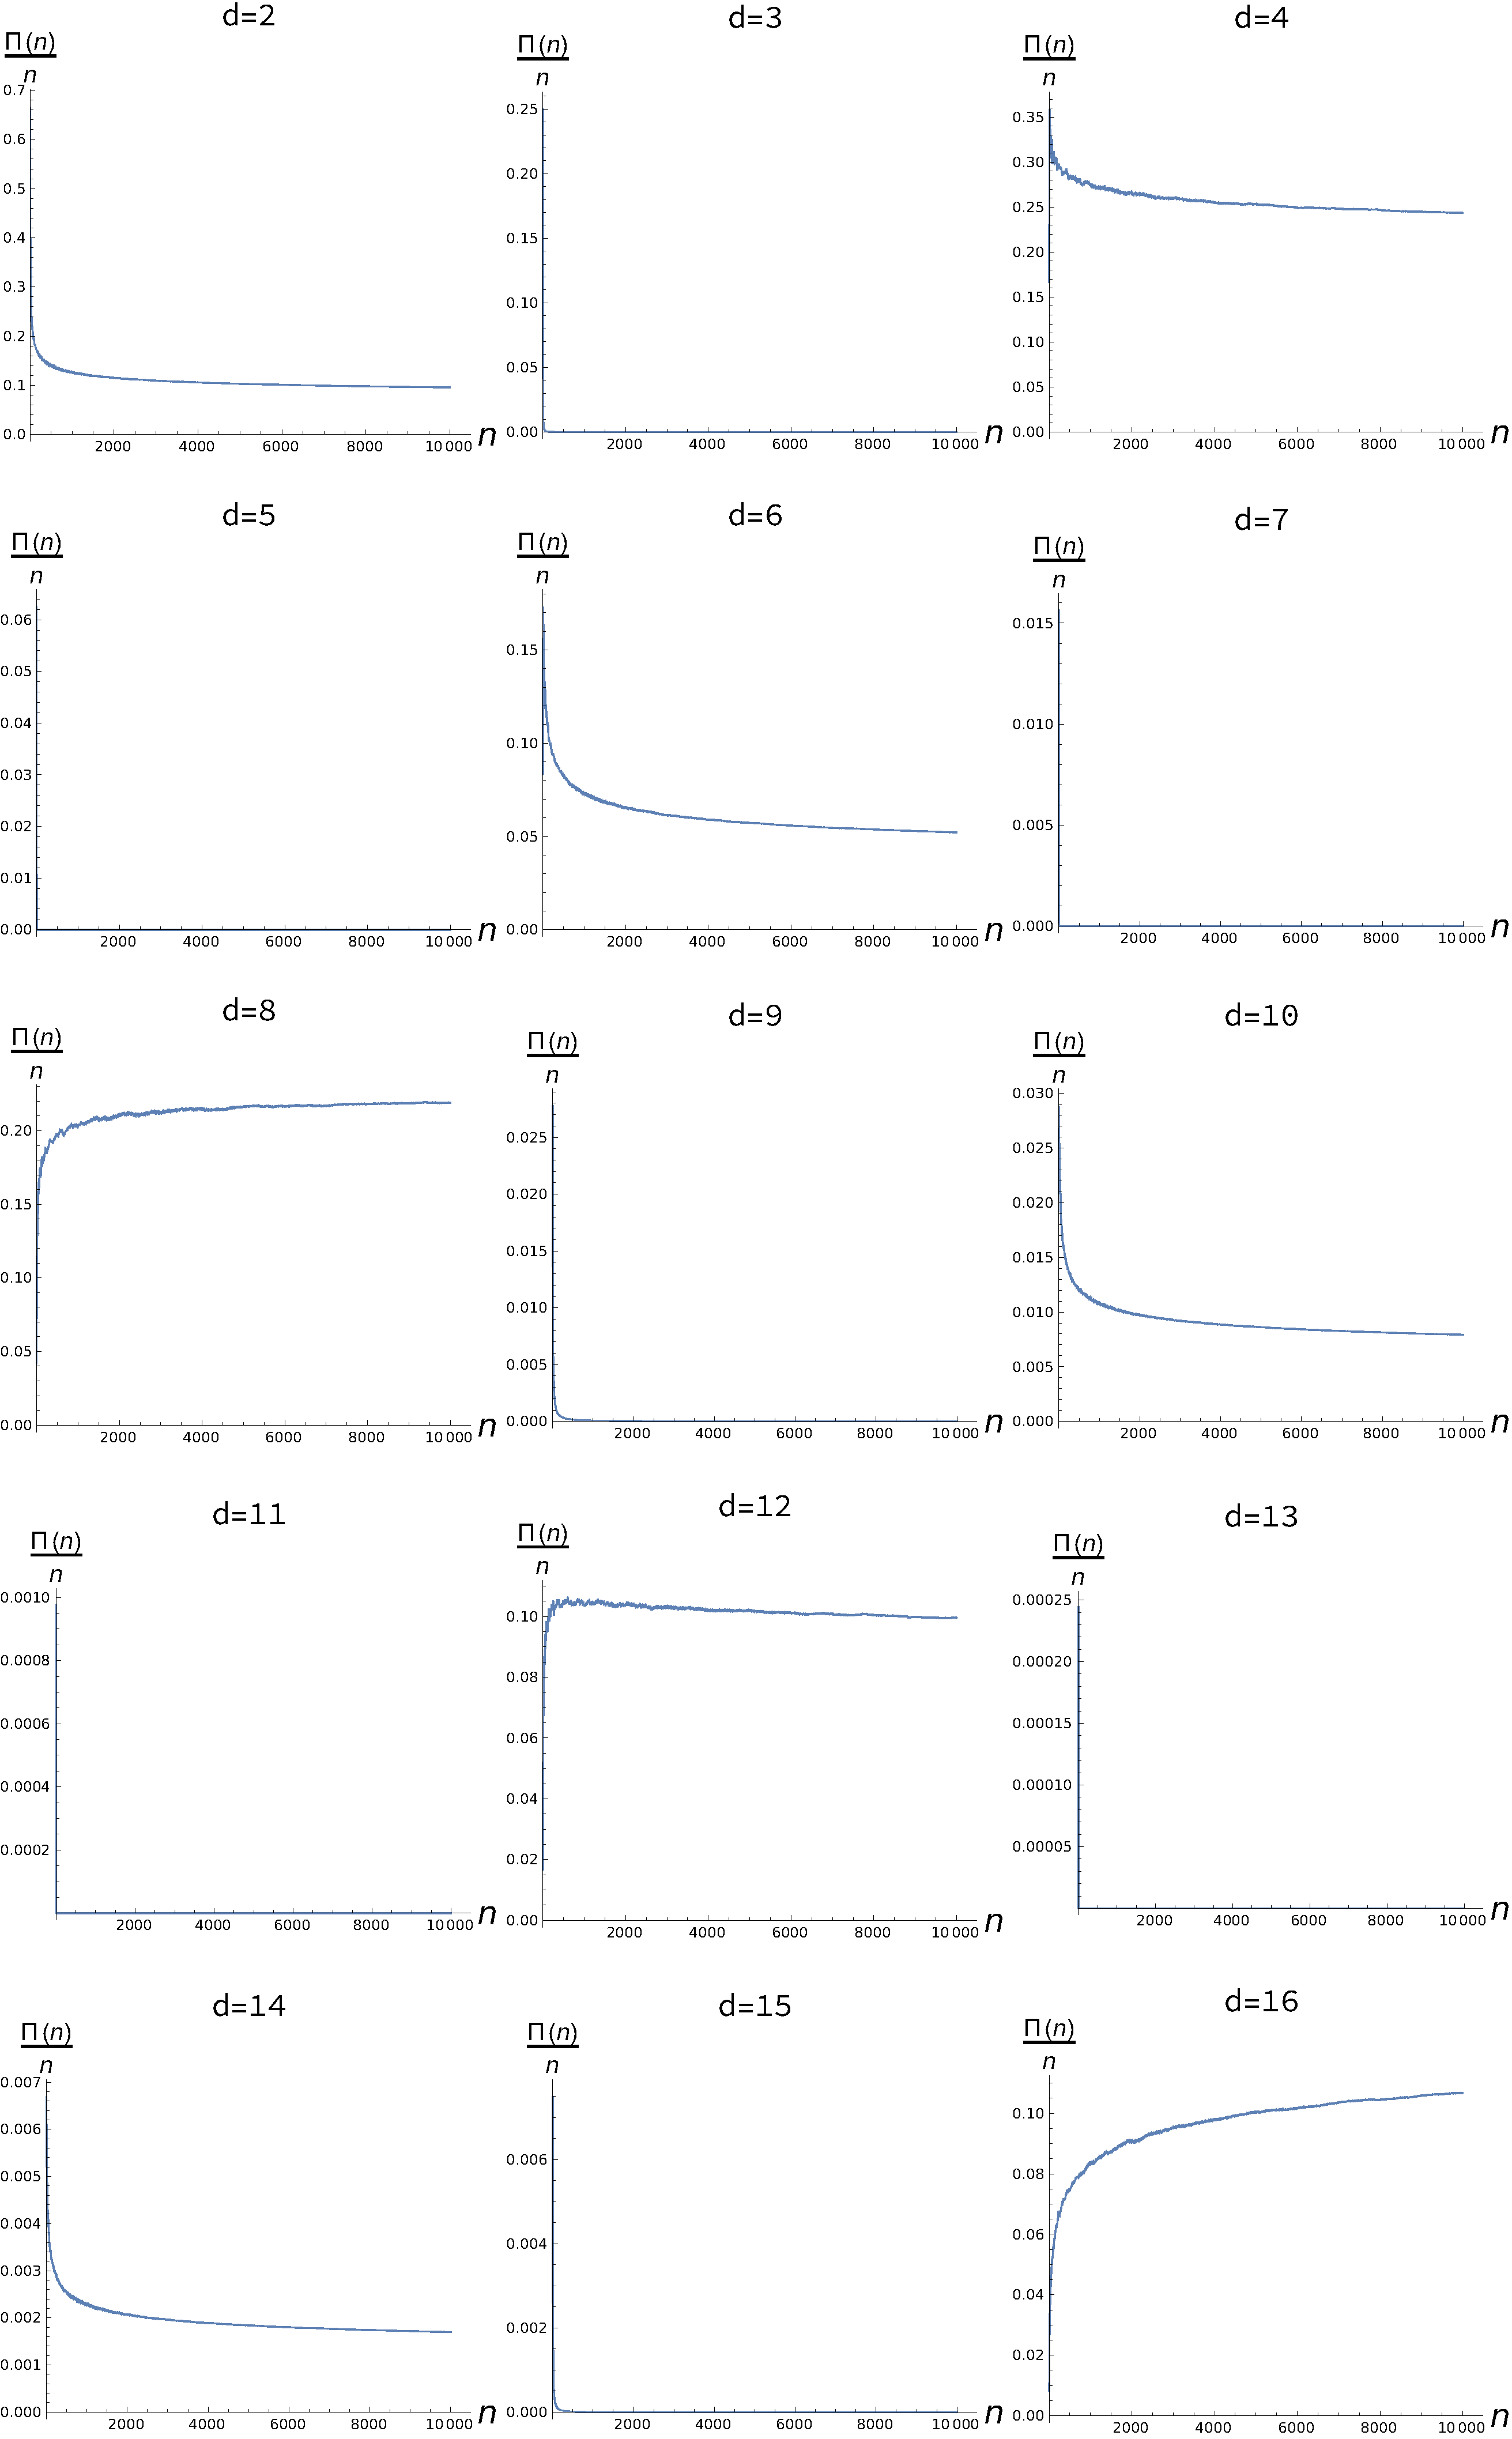
\includegraphics[width=0.86\textwidth]{Images/counts.pdf}
    \caption{Densidades de $d$-primos para $d=2,3,\ldots, 11$. No eixo horizontal
    estão os inteiros e no vertical o valor de $\Pi_d(n)/n$: a quantidade
    de $d$-primos em relação à $n$.}
    \label{graph-counts}
\end{figure}

\section{Quantidade de divisores dos naturais}

Nesta seção, relatam-se os resultados referentes aos grafos
gerados usando a sequência de divisores e a sequência das órbitas dos divisores, definidas na Seção 3.3.

A Tabela 4.4 reúne os dados da função $Ak^{-\gamma}$ que ajusta a distribuição de graus $P(k)$ dos grafos de VH e VN.


\begin{table}[H]
    \centering
    \caption{Valores de $A$ e $\gamma$ para os grafos de VH e VN.}
    \begin{tabular}{|c|c|c|c|c|}
        \hline série & visibilidade & $\langle k \rangle$ & $\gamma$ & $A$ \\
        \hline
        divisores & natural & 5.6 & $1.2 \pm 0.2$ & $0.56 \pm 0.13$ \\
        divisores & horizontal & 3.6 & $0.64 \pm 0.66$ & $0.19 \pm 0.17$ \\
        órbitas & natural & 4.9 & $0.56 \pm 0.41$ & $0.15 \pm 0.10$ \\
        órbitas & horizontal & 3.0 & $0.3 \pm 1.6$ & $0.20 \pm 0.39$ \\
         \hline 
    \end{tabular}
    \label{tab:div-orb}
\end{table}

Nota-se que o valor de $\gamma$ para a sequência das órbitas é aproximadamente metade
do valor de $\gamma$ para a sequência de divisores.

\subsection{Sequência de divisores}

A Figura 4.4 mostra o grafo gerado a partir de um número $x$ e sua quantidade de divisores $D(x)$, isto é, o grafo com conexões $x\to D(x)$.

\begin{figure}[H]
    \centering
    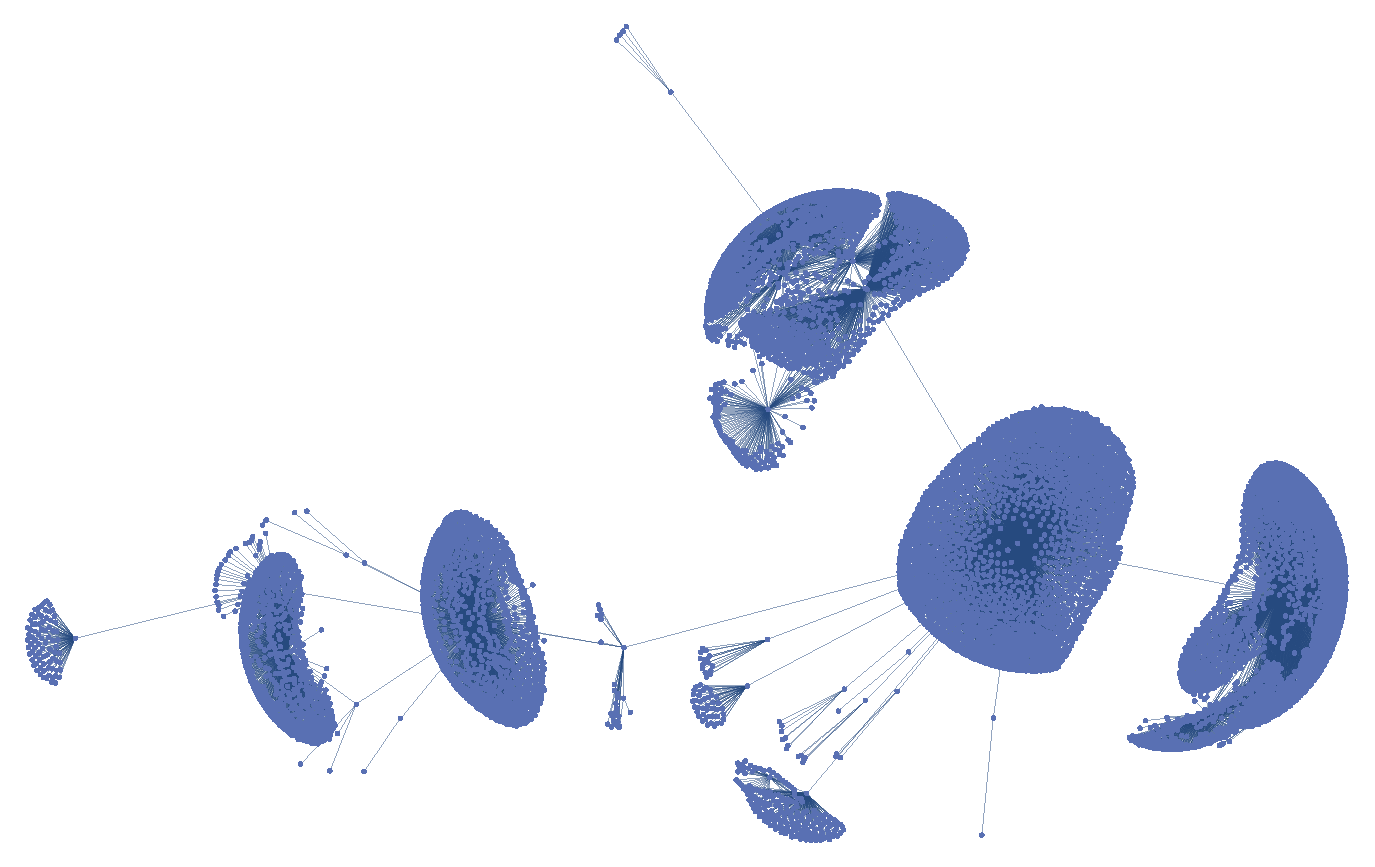
\includegraphics[width=0.65\textwidth]{article-2/divisors.pdf}
    \caption{Grafo gerado usando a sequência dos divisores. As ligações são estabelecidas entre um número
    e sua quantidade de divisores; por exemplo: $4\to 3$, $5\to 2$ e $10\to 4$.}
    \label{graph-divs}
\end{figure}

Essa mesma sequência foi usada para gerar os grafos de VN e VH. A Figura 4.5 mostra os grafos gerados utilizando os dois algoritmos de visibilidade para uma sequência com
apenas os 100 primeiros números  (números maiores dificultam a visualização). Como esperado, no grafo de VH existem menos conexões do que no de VN. Entretanto, nas análises foram considerados mais números.

\begin{figure}[H]
    \centering
    \includegraphics[width=0.95\textwidth]{article-2/divisors-vis-graphs.pdf}
    \caption{Grafos gerados usando os dois algoritmos de visibilidade. Esquerda: visibilidade natural; 
    direita: visibilidade horizontal.}
    \label{graph-divs-vis}
\end{figure}

Os grafos gerados por essas sequências reflete um grafo mais fortemente conectado se comparado
ao grafo da sequencia das orbitas. E o que também é observado no grau médio.

A Figura 4.6 mostra a variação do caminho mínimo médio $\langle l\rangle$ em função da quantidade de nós $n$. Aparentemente, essa curva converge para $\langle l\rangle \simeq 4$.

\begin{figure}[H]
    \centering
    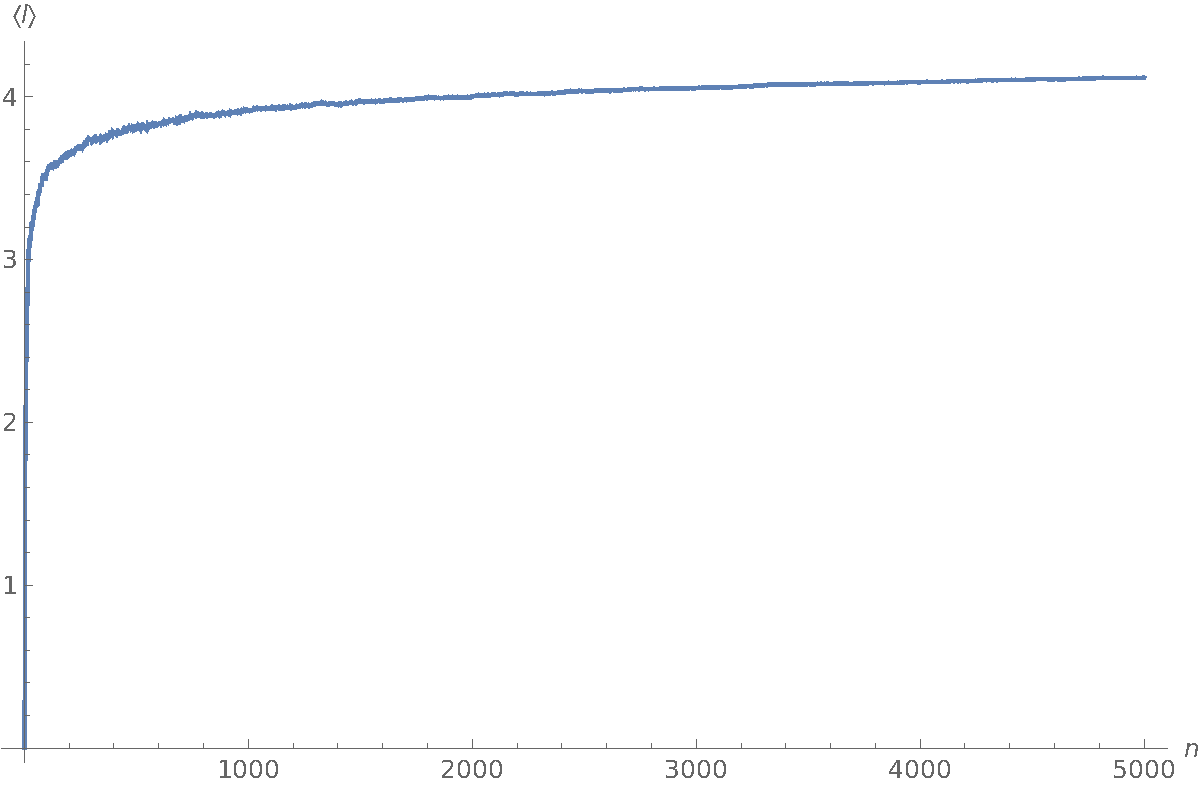
\includegraphics[width=0.9\textwidth]{article-2/growth-divisors.pdf}
    \caption{Caminho mínimo médio $\langle l\rangle$ em função da quantidade de nós $n$, calculado até 5000 nós para a sequência
    dos divisores.}
    \label{graph-growth}
\end{figure}

Entretanto, uma análise mais atenta da Figura 4.6 revela que $\langle l\rangle$
não para de crescer, pois  suas
casas decimais não convergem. O cálculo de $\langle l\rangle$ pode ser útil no estudo
das lacunas entre os $d$-primos, pois esse valor pode ser usado como heurística para a determinação
de limites superior e inferior dessas lacunas.


\subsection{Sequência das órbitas}

A Figura 4.7 mostra o grafo obtido considerando a sequência das órbitas.

\begin{figure}[H]
    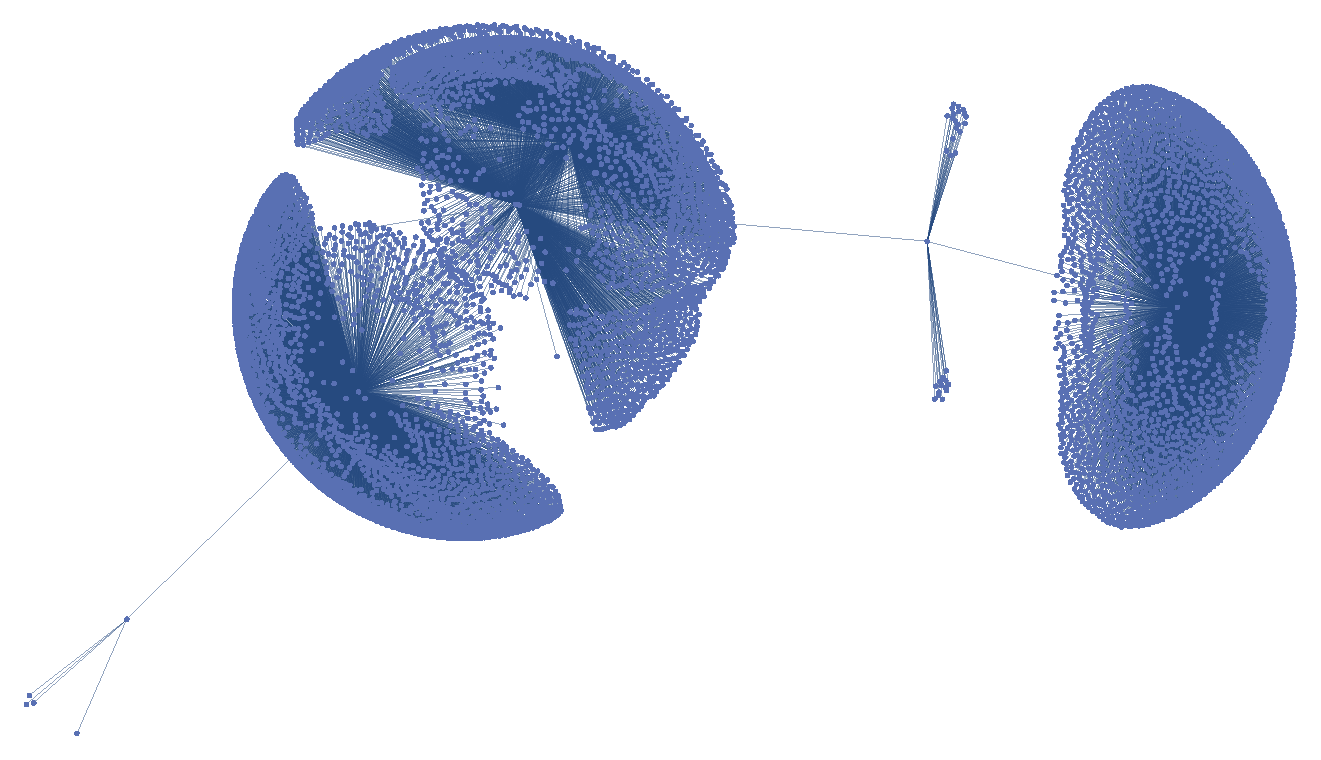
\includegraphics[width=0.65\textwidth]{article-2/orbits.pdf}
    \centering
    \caption{Grafo gerado usando a sequência das órbitas. Por exemplo, há a conexão $10\to3$, pois 10 tem 4 divisores, 4 tem 3 divisores e 3 tem 2 divisores. Como
    a contagem de divisores foi feita 3 vezes, cria-se a ligação entre 10 e 3.}
    \label{frame}
\end{figure}

O grafo apresenta estrutura similar ao encontrado na sequencia de divisores, possui centros
com muitas ligações e ligações com outros centros, o que confere a estrutura de árvore a ambos.

Porém os centros são mais evidentes neste estudo, por sua menor quantidade.


A Figura 4.8 mostra os grafos de VN e VH com apenas 100 números.

\begin{figure}[H]
    \centering
    \includegraphics[width=0.9\textwidth]{article-2/orbits-vis-graphs.pdf}
    \caption{ Grafos gerados usando os algoritmos de visibilidade. Esquerda: visibilidade natural; 
    direita: visibilidade horizontal.}
    \label{graph-orbits-vis}
\end{figure}

Os grafos mostram maior número de conexões em poucos nós, isto é, menor variedade.
Apesar de similares, é possível perceber uma diferença na quantidade das
conexões $1\to 1$ e $3\to 3$. 
A Figura 4.9 mostra a variação do caminho mínimo médio em relação ao
número de nós.

\begin{figure}[H]
    \centering
    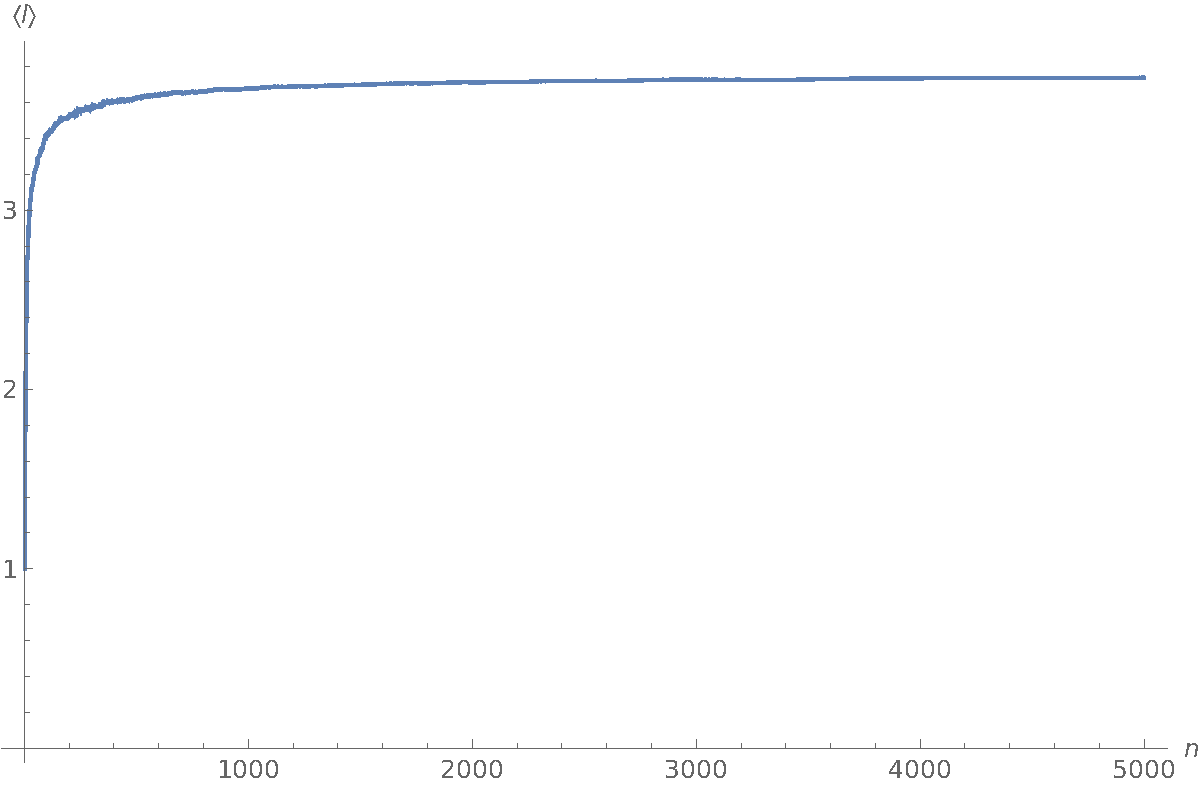
\includegraphics[width=0.9\textwidth]{article-2/growth-orbits.pdf}
    \caption{Caminho mínimo médio $\langle l\rangle$ em função da quantidade de nós $n$, calculado até 5000 nós para a sequencia das órbitas.}
    \label{means}
\end{figure}

Nessa sequência o caminho mínimo médio se estabiliza num valor de forma mais rápida, atingindo o
valor $3.73921$ para 5000 números.


\section{Casas decimais de números irracionais}

Para cada número irracional considerado, foram geradas sequências que foram transformadas em
grafos utilizando-se os algoritmos de visibilidade.

A Tabela 4.5 mostra os valores numéricos das propriedades dos grafos de VN e VH, além da entropia normalizada $h$ e da complexidade SDL.

\begin{table}[H]
    \small
    \centering
    \caption{ Propriedades dos grafos gerados a partir de números irracionais.}
    \begin{tabular}{|c|cc|ccc|ccc|}
    \hline
 &&& \multicolumn{3}{|c|}{Visibilidade Natural} & \multicolumn{3}{|c|}{Visibilidade Horizontal} \\
& $C_{SDL}$ & $h$ & $\langle k \rangle$ & $A$ & $\gamma$  & $\langle k \rangle$ & $A$ & $\gamma$ \\
\hline 
 $\sqrt{2}$     & 0.194 & 0.948 & 5.19 & 0.70$\pm$0.13 & 1.34$\pm$0.16 & 3.63 & 1.33$\pm$0.26 & 1.73$\pm$0.20 \\
 $\sqrt{2}_2$   & 0.135 & 0.964 & 5.40 & 0.65$\pm$0.12 & 1.30$\pm$0.15 & 3.95 & 1.21$\pm$0.17 & 1.69$\pm$0.14 \\
 $\sqrt{2}_3$   & 0.097 & 0.975 & 5.39 & 0.66$\pm$0.12 & 1.31$\pm$0.15 & 3.99 & 1.21$\pm$0.16 & 1.69$\pm$0.13 \\
 $\phi$         & 0.192 & 0.949 & 5.21 & 0.69$\pm$0.13 & 1.33$\pm$0.17 & 3.63 & 1.32$\pm$0.26 & 1.73$\pm$0.21 \\
 $\phi_2$       & 0.136 & 0.964 & 5.37 & 0.66$\pm$0.12 & 1.31$\pm$0.15 & 3.95 & 1.22$\pm$0.17 & 1.69$\pm$0.15 \\
 $\phi_3$       & 0.096 & 0.975 & 5.37 & 0.66$\pm$0.13 & 1.31$\pm$0.16 & 3.99 & 1.20$\pm$0.17 & 1.68$\pm$0.14 \\
 $e$            & 0.195 & 0.948 & 5.21 & 0.69$\pm$0.13 & 1.33$\pm$0.16 & 3.64 & 1.33$\pm$0.24 & 1.73$\pm$0.19 \\
 $e_2$          & 0.149 & 0.961 & 5.35 & 0.65$\pm$0.13 & 1.30$\pm$0.16 & 3.94 & 1.22$\pm$0.17 & 1.69$\pm$0.14 \\
 $e_3$          & 0.096 & 0.975 & 5.35 & 0.67$\pm$0.12 & 1.32$\pm$0.15 & 3.99 & 1.22$\pm$0.15 & 1.69$\pm$0.13 \\
 $\pi$          & 0.192 & 0.949 & 5.19 & 0.70$\pm$0.13 & 1.34$\pm$0.16 & 3.64 & 1.33$\pm$0.25 & 1.73$\pm$0.19 \\
 $\pi_2$        & 0.145 & 0.962 & 5.38 & 0.65$\pm$0.12 & 1.30$\pm$0.16 & 3.95 & 1.21$\pm$0.17 & 1.68$\pm$0.14 \\
 $\pi_3$        & 0.100 & 0.974 & 5.37 & 0.66$\pm$0.14 & 1.31$\pm$0.15 & 3.99 & 1.20$\pm$0.17 & 1.68$\pm$0.15 \\
 \hline
\end{tabular}
    \label{tab:numbers}
\end{table}

Para todas as sequências analisadas, os valores de $h$, $\langle k\rangle$, $A$ e $\gamma$ são muito próximos.

Sabe-se que distribuições uniformes podem estar relacionadas à aleatoriedade \cite{avigad_2013}. A Figura 4.10 mostra histogramas da frequência relativa de cada número, par ou tripla em cada sequência analisada.

\begin{figure}[H]
    \centering
    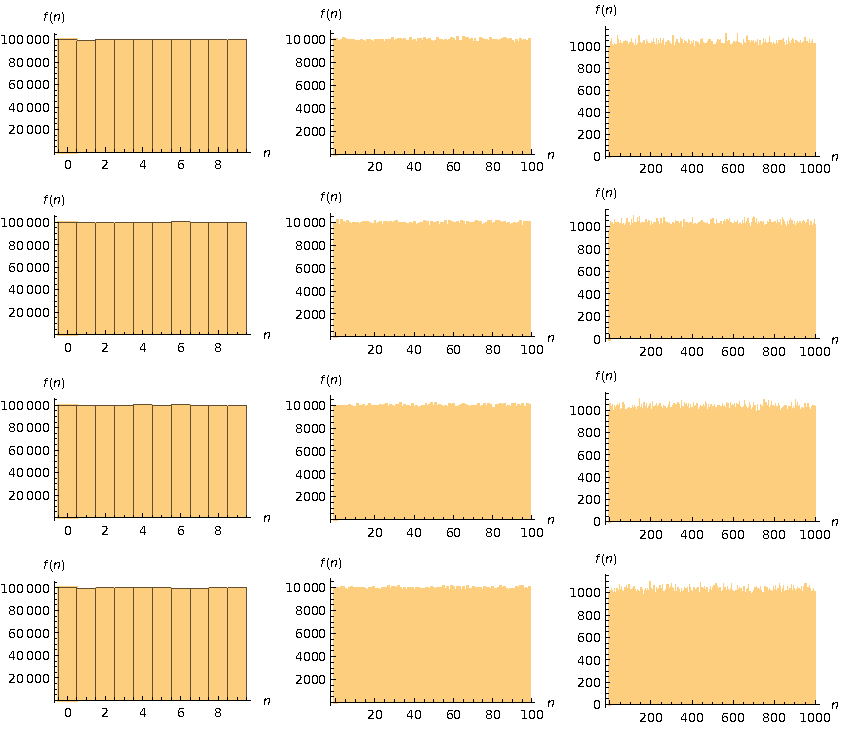
\includegraphics{article-2/numbers-dist.pdf}
    \caption{Histogramas das frequências dos dígitos. De cima para baixo: 
    $\sqrt{2}, \phi, e, \pi$. Da esquerda para a direita: dígitos únicos, pares e triplas.
    No eixo horizontal $n$ é o número, par ou tripla da sequência e o eixo vertical a 
    frequencia encontrada, representada por $f(x)$.}
    \label{histograms}
\end{figure}

As distribuições são uniformes para todos os casos, o que é uma característica
de números uniformemente aleatórios.

No próximo capítulo, apresentam-se comentários e conclusões a partir dos resultados mostrados neste capítulo.


\chapter{DISCUSSÃO E PRÓXIMOS PASSOS}





\section{Lacunas entre $d$-primos}

Como mostra a Tabela 4.1, $h \simeq 1$ para
$d=\{3,5,7,9,11\}$, pois repetições nas sequencias de $x_d$ são
 raras, ou seja, essas sequencias são aperiódicas.
Adicionalmente $h \approx 0.7$ para $d=\{2,4,6,8,10\}$, 
então a variabilidade do tamanho das lacunas para $d$ par é
menor do que para $d$ impar. Então uma possível conjectura é:
a entropia normalizada $h$ distingue $d$ par ($h \approx 0.7$)
de $d$ impar ($h\simeq 1$) \cite{me_2020}.

As Figuras 4.1 e 4.2 e as Tabelas
4.2 e 4.3 mostram que a maior parte
das distribuições de graus $P(k)$ dos grafos de VN e VH construídos a partir
das lacunas entre $d$-primos sucessivos para $d \in \{2, 3, \ldots, 11\}$
segue, aproximadamente, uma lei de potências dada por $P(k)=A k^{-\gamma}$.
As flutuações observadas próximas às linhas retas mostradas nessas figuras
podem ser causadas pelo tamanho finito das sequências $x_d$ usadas nos
estudos numéricos \cite{li2}.  Distribuições que seguem uma lei de potência
na conectividade $P(k)$ estão associadas com redes complexas conhecidas como
livres de escala \cite{li2,a81,a83}. A invariância de escala na distribuição
de graus $P(k)$ implica autossimilaridade, isto é, $P(k)$ de redes renormalizadas,
obtidas por um processo de empacotamento \cite{a400}, também seguem uma lei
de potência.

Nota-se que o valor de $\gamma$ nos gráficos de VN e VH não é um bom parâmetro
para mostrar a influência do valor de $d$ nas redes geradas pelas sequencias
de lacunas; entretanto $\langle k \rangle$ pode mostrar essa influência. De fato, nos gráficos de VN, para $d$
primo, $\langle k \rangle$ aumenta com $d$; para $d$ não primo,
$\langle k \rangle \approx 6$; nos gráficos de VH, $\langle k \rangle >
3.90$ para $d$ impar e $\langle k \rangle < 3.90$ para $d$ par.
Portanto, outra conjectura possível é: $\langle k \rangle$ distingue
$d$ primos dos $d$ não primos para a VN; e $\langle k \rangle$ distingue
$d$ impar de $d$ par nos gráficos de VH \cite{me_2020}..

É sabido que para grafos de VH obtidos de sequencias periódicas de período
$T$ (sem números repetidos dentro de um período), o grau médio é dado por
$\langle k \rangle = 4[1-(1/(2T)]$ \cite{a310}. Como consequência, para
sequências aperiódicas, $\langle k \rangle = 4$ (pois $T \to \infty$).
Na Tabela 4.3, esse é o valor aproximado de
$\langle k \rangle$ encontrado para $d$-primos com $d$ impar, o que está
de acordo com o valor de $h$ apresentado na tabela 4.1.
Também é conhecido que para uma sequência não correlacionada aleatória,
o grafo de VH tem $P_{rand}(k)= (1/3)(2/3)^{k-2}$ \cite{a310}. Portanto, 
desvios dessa distribuição de graus revelam que a sequência estudada não
foi gerada por um processo aleatório não correlacionado. A curva correspondente
a $P_{rand}(k)$ é mostrada como uma linha pontilhada na Figura 4.2.
Note que $P(k)$ para $d$-primos tem menor inclinação do que $P_{rand}(k)$.
Essa menor inclinação e $\langle k \rangle = 4$ podem ser indicações de
uma sequência caótica \cite{a310}.


\section{Densidade de $d$-primos}

Nota-se na Figura 4.3 que existe uma distinção de comportamento na densidade dos $d$-primos:
para $d$ par, a densidade tende a um número fixo pequeno, entre 0.005 e 0.3;
para $d$ impar, esses valores caem rapidamente e se aproximam de zero.

Dentre os pares, apenas para $d=8$ a densidade tem concavidade voltada para baixo; para as demais curvas com $d$ par, a densidade tem concavidade voltada para cima. Esse é o comportamento dos números primos usuais, ou seja, do caso em que $d=2$. Esse resultado para $d=2$ já era conhecido. Pode-se conjecturar que a dependência da densidade $\Pi_d(n)/n$ com $n$  para outros valores pares de $d$ é similar ao caso $d=2$.




\section{Quantidade de divisores dos naturais}

A sequência de divisores e a sequência das órbitas dos divisores levaram a grafos de VN e VH em que
$P(k) = A k^{-\gamma}$; ou seja, $P(k)$ segue uma lei de potência. Portanto, esses  grafos são livres de escala.
Além disso, o  coeficiente $\gamma$ para a sequência das órbitas 
é aproximadamente metade daquele relacionado à sequência dos divisores.

%% explicar o fato de <l>(n) convergir e não convergir. O que isso diz sobre o grafo?

%Os valores de $C$ e $\gamma$ para a sequência de divisores são muito próximos dos
%mesmos coeficientes da sequência de diferença entre números primos, como foi explorado
%em \cite{me_2020}.

%Na sequência das órbitas o caminho mínimo médio convergiu para o valor $3.73921$. Usar sequências
%maiores pode aumentar a precisão dos resultados, porém devido ao poder computacional
%foram utilizados apenas 10000 números. Além disso a convergência do caminho mínimo médio
%dos divisores não foi notada, pois para 10 mil números o valor é $4.19149$; para 15 mil, $4.24815$;
%e para 18 mil, $4.25646$.



\section{Casas decimais de números irracionais}

Os histogramas aproximadamente constantes mostrados na Figura 4.10 sugerem
uma aleatoriedade uniforme
dos dígitos que compõem as casas decimais dos números  considerados.

Como observado na Tabelas 4.5, os valores de $\langle k \rangle$, $A$ e $\gamma$ são muito próximos para todos oa grafos construídos.
Pode-se conjecturar que
os dois algoritmos de visibilidade não diferenciam números transcendentais
dos irracionais.
Entretanto, a complexidade SDL cai conforme se aumenta a quantidade de dígitos que formam as sequências. Para os quatro números considerados, o valor de $C_{SDL}$ para sequências com único dígito é maior que para sequências com pares de dígitos que é maior para sequências com triplas de dígitos.



\section{Observações finais}

Nota-se sobre os estudos de visibilidade de $n$-primos e da sequencia de divisores
que possuem valores próximo para casos específicos, por exemplo o valor de $\gamma$
aproximadamente 1.2, que se repete algumas vezes também é o valor de $\gamma$ para
a visibilidade natural da sequencia dos divisores.

Além disso as sequencias de $d$-primos, na visibilidade natural, possuem valores ligeiramente diferentes das sequencias de dígitos de números irracionais; porém na visibilidade horizontal possui valores próximos, 1.7.



\section{Trabalhos futuros}

O prazo final para a entrega desta tese é meados de 2023.

Os estudos sobre divisores dos naturais e sobre números irracionais ainda carecem de melhor análise, é necessário estudar mais números e utilizar sequências maiores. Talvez se possa analisar as sequências geradas quando se escreve um número irracional $y$ como uma fração contínua, ou seja, quando se escreve tal número da seguinte forma:
\begin{equation*}
 y = a_0 + \frac{1}{a_1+\frac{1}{a_2+ \frac{1}{a_3+...}}}    
\end{equation*}

\noindent A sequência $\{a_0,a_1,a_2,...\}$ caracteriza $y$. Por exemplo, para o número $\phi$, tem-se $a_j=1$ para todo $j$.

O uso de algoritmos de visibilidade em sequências de dígitos derivadas de números
racionais ainda não foi investigado. Pode ser interessante comparar os resultados de números irracionais
com os resultados de números racionais.

Nos estudos sobre as densidades de $d$-primos, a convergência pode ser determinada e relacionada
com os valores encontrados para os números primos. Outra investigação possível é verificar a 
relação das densidades com as diferenças entre os $d$-primos.

Um ponto de estudo usando os algoritmos de visibilidade nos estudos de lacunas entre $d$-primos
é procurar os valores de máximo e mínimo de intervalos utilizando as propriedades desses grafos,
por exemplo, o caminho mínimo médio e o coeficiente de agregação.


\def \label{REFERÊNCIAS BIBLIOGRÁFICAS}
%\bibliographystyle{abbrv}
\bibliography{biblproj}
\addcontentsline{toc}{section}{REFERÊNCIAS BIBLIOGRÁFICAS}
\bibliographystyle{abnt-alf}
\end{document}